\documentclass[norsk,a4paper,11pt]{article}
\usepackage[T1]{fontenc} %for å bruke æøå
\usepackage[utf8]{inputenc}
\usepackage{amsmath, amsfonts, amssymb}
\usepackage{graphicx} %for å inkludere grafikk
\usepackage{verbatim} %for å inkludere filer med tegn LaTeX ikke liker
\usepackage{mathpazo}
\usepackage[font=scriptsize]{caption}
\bibliographystyle{plain}


\title{Computing correlation energy with Gauss Quadrature and Monte Carlo \\ FYS3150 Project 2}
\author{Vilde Flusgrud}
\begin{document}
\date{\today}
\maketitle

\begin{abstract}
    This project applies Gaussian Quadrature and Monte Carlo integration methods to numerically solve the six-dimensional integral
    which determines the ground state correlation energy between two electrons in the Helium atom. Specifically this project aims to
    investigate the effect of optimizing the brute force methods with more advanced techniques. I find that a Monte Carlo method
    using importance sampling and the exponential distribution is the best fit, achieving a precision of 5 leading digits for $N=10^6$
    in a couple of seconds.
\end{abstract}
    

\section{Introduction}
The integral we aim to compute is a six dimensional integral which determine the ground state correlation energy
between two electrons in a Helium atom. In general the correlation energy is hard or impossible to compute analytically.
It is therefore of interest to investigate how to best solve the problem numerically.

I have tested two different integration techniques, Gaussian Quadrature and Monte Carlo, in both cases started with a brute force
method and proceeded to more advanced solutions. The work done includes rewriting our integral
in forms that let us use the properties of certain polynomials and probability distributions, as well as implementing the algorithms
in c++ programs and evaluating the results.

The report consists of a method section which gives the backround of the methods and a result section which presents the output. Programs
and output examples are found at https://github.com/vildemf/compphys in the project 3 folder. The relevant programs are main.cpp and
methods.cpp.

\section{Method}
We assume that the wave function of each electron can be modelled like the single-particle
wave function of an electron in the hydrogen atom. The single-particle wave function for an electron $i$ in the
$1s$ state
is given in terms of a dimensionless variable (the wave function is not properly normalized)
\begin{align}
    {\bf r}_i = x_i {\bf e}_x + y_i {\bf e}_y +z_i {\bf e}_z ,
\end{align}
as
\begin{align}
\psi_{1s}({\bf r}_i) = e^{-\alpha r_i},
\end{align}
where $\alpha$ is a parameter and
\begin{align}
r_i = \sqrt{x_i^2+y_i^2+z_i^2}.
\end{align}
We will fix $\alpha=2$, which should correspond to the charge of the helium atom $Z=2$.
The ansatz for the wave function for two electrons is then given by the product of two
so-called
$1s$ wave functions as
\begin{align}
\Psi({\bf r}_1,{\bf r}_2) = e^{-\alpha (r_1+r_2)}.
\end{align}

The integral we need to solve is the quantum mechanical expectation value of the correlation
energy between two electrons which repel each other via the classical Coulomb interaction, namely
\begin{equation}\label{eq:correlationenergy}
\langle \frac{1}{|{\bf r}_1-{\bf r}_2|} \rangle =
\int_{-\infty}^{\infty} d{\bf r}_1d{\bf r}_2 e^{-2\alpha (r_1+r_2)}\frac{1}{|{\bf r}_1-{\bf r}_2|}.
\end{equation}
Note that our wave function is not normalized. There is a normalization factor missing, but for this project
we don't need to worry about that.
This integral can be solved in closed form and the answer is $5\pi^2/16^2$. This solution is useful for evaluating our
numerical results.
\subsection{Gaussian Quadrature}
Numerical integration algorithms in the simplest form generate mesh points as 
$N$ $x$-values with equal spacing. The integrand is then interpolated by a polynomal of at most
degree $N - 1$. Gaussian Quadrature however is a more complex method which is able to achieve a greater precision
for a given amount of numerical work - we can represent the integrand with a polynomial of degree $2N-1$ and still only
have $N$ points. The idea of GQ is to not require
equal spacing, but start by rewriting the integrand as
\begin{align}
    I = \int_a^b f(x) \mathrm{d}x = \int_a^b W(x) g(x) \mathrm{d}x \approx \sum_{i=1}^{N} \omega_i g(x_i)
\end{align} 

where $W$ must be a weight function associated with a given orthogonal polynomial. Extracting such a $W$ from
our integrand $f$, we use it to compute weights
$\omega_i$ and end up only evaluating the integral for the function $g$, which is smooth.
The mesh points $x_i$ are then chosen in some optimal sense, the only constraint being it has to stay within the interval 
for which the given polynomial is orthogonal. In this project we look at the Legendre and Laguerre polynomials, for which $W$ and
the orthogonal interval is given in table \ref{tab:m1}.

\begin{table}
  \begin{center}
  \caption{
      \label{tab:m1}
  Weight functions and orthogonal intervals for the Legendre and Laguerre polynomials}
  \begin{tabular}{|c|c|c|} \hline
      \textbf{Polynomial} & \textbf{Weight function $W(x)$} & \textbf{Orthogonal interval} \\ \hline
      Legendre  &  $1$ & $x \in [-1, 1]$\\
      Laguerre & $x^\alpha e^{-x}$ & $0 \leq x \leq \infty $  \\ \hline
  \end{tabular}
  \end{center}
\end{table}


\subsubsection{Brute force: Gauss-Legendre}
Our first approach is a brute force GQ integration method using the Legendre polynomials. We wish to compute

\begin{align*}
     I & = 
    \int_{-\infty}^{\infty} d{\bf r}_1d{\bf r}_2 e^{-2\alpha (r_1+r_2)}\frac{1}{|{\bf r}_1-{\bf r}_2|} \\
    & = \int_{-\infty}^{\infty} \int_{-\infty}^{\infty} \int_{-\infty}^{\infty} \int_{-\infty}^{\infty} \int_{-\infty}^{\infty} \int_{-\infty}^{\infty}
      e^{-2\alpha (r_1+r_2)}\frac{1}{|{\bf r}_1-{\bf r}_2|}
     \mathrm{d}x_1 \mathrm{d}x_2 \mathrm{d}y_1 \mathrm{d}y_2 \mathrm{d}z_1 \mathrm{d}z_2 \\
    & \approx
    \int_{a}^{b} \int_{a}^{b} \int_{a}^{b} \int_{a}^{b} \int_{a}^{b} \int_{a}^{b}
      e^{-2\alpha (r_1+r_2)}\frac{1}{|{\bf r}_1-{\bf r}_2|}
     \mathrm{d}x_1 \mathrm{d}x_2 \mathrm{d}y_1 \mathrm{d}y_2 \mathrm{d}z_1 \mathrm{d}z_2
\end{align*}
Where the $\infty$-limits need to be approximated in order to make the problem computer friendly. In order to choose approporiate 
approximate limits $a$ and $b$ we look at how our model for the wave function of each particle,
$\psi_{1s}({\bf r}_i) = e^{-\alpha r_i}$, behaves in the limits. See the plot in figure \ref{fig:m1}.

\begin{figure}
    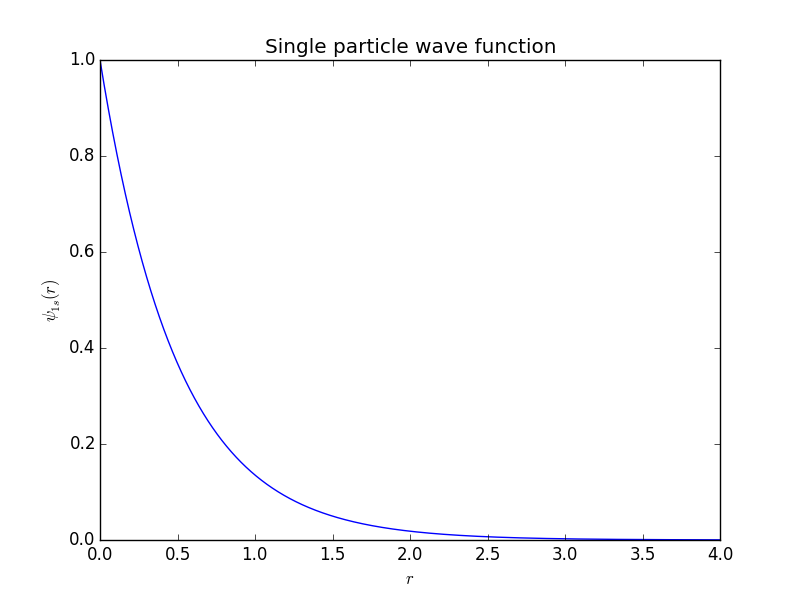
\includegraphics[width=0.9\linewidth]{m1.png}
    \caption{
        \label{fig:m1}
    Plot of the wave function for one electron in order to observe where it goes to zero. The wave function is 
    modelled by the single-particle wave function of an electron in the hydrogen atom, $\psi_{1s}(r_i) = e^{-\alpha r_i}$.}
\end{figure}

We see that it approaches zero around $r=3.0$ and set the limits to $a=-3$ and $a=3$. We know the Legendre polynomials only stay
orthogonal on the interval $x\in [-1, 1]$. The algorithm solves this by a change of variables.
Since for Legendre we have $W(x) = 1$ we do not have to rewrite our integrand. Thus our procedure will be a call to a function
(gauleg(), a course library function) which generates weights $\omega_i$ and integration points $x_i$, followed by
a six-double for-loop to compute all values of the integrand and add to the total sum.
We need to decide how to handle the case where $|{\bf r}_1 - {\bf r}_2|$ approach zero.
Physically this corresponds to the two electrons being in the same place, which cannot happen. Thus we ignore these terms of the sum
by returning zero.

\subsubsection{Improved: Gauss-Legendre and Gauss-Laguerre}
We wish to improve the method and change our integral from cartesian to spherical coordinates. This gives

\begin{align*}
    I & =\int_{0}^{\infty} \int_{0}^{\infty} \int_{0}^{2\pi} \int_{0}^{2\pi} \int_{0}^{\pi} \int_{0}^{\pi}
      e^{-2\alpha (r_1+r_2)}\frac{1}{r_{12}} r_1^2 r_2^2 sin\theta_1 sin\theta_2
     \mathrm{d}\theta_1 \mathrm{d}\theta_2 \mathrm{d}\phi_1 \mathrm{d}\phi_2 \mathrm{d}r_1 \mathrm{d}r_2  
\end{align*}

Where
\begin{align}
     \frac{1}{r_{12}} = \frac{1}{|{\bf r}_1-{\bf r}_2|} = \frac{1}{\sqrt{r_1^2+r_2^2-2r_1r_2cos(\beta)}}
\end{align}
with

\begin{align}
    cos(\beta) = cos(\theta_1)cos(\theta_2)+sin(\theta_1)sin(\theta_2)cos(\phi_1-\phi_2))
\end{align}

For $\theta$ and $\phi$ we use the Legendre polynomials to generate $\omega_i$'s as before, with limits $a=0$ and $b=\pi$
and $b=2\pi$ respectively.
For the $r$'s on the other hand we see that the interval now corresponds to the orthogonal interval of the Laguerre
polynomials. We make a substitution $u = 2\alpha r$ in order get our integrand on a form where we can extract the Laguerre $W$.
This substitution gives us

\begin{align*}
     I &= (2\alpha)^{-5}\int_{0}^{\infty} \int_{0}^{\infty} \int_{0}^{2\pi} \int_{0}^{2\pi} \int_{0}^{\pi} \int_{0}^{\pi}
      e^{-(u_1+u_2)}\frac{1}{u_{12}} u_1^2 u_2^2 sin\theta_1 sin\theta_2
     \mathrm{d}\theta_1 \mathrm{d}\theta_2 \mathrm{d}\phi_1 \mathrm{d}\phi_2 \mathrm{d}u_1 \mathrm{d}u_2 \\
      & = (2\alpha)^{-5}\int_{0}^{\infty} \int_{0}^{\infty} \int_{0}^{2\pi} \int_{0}^{2\pi} \int_{0}^{\pi} \int_{0}^{\pi}
      W(u_1)W(u_2)\frac{1}{u_{12}} sin\theta_1 sin\theta_2
     \mathrm{d}\theta_1 \mathrm{d}\theta_2 \mathrm{d}\phi_1 \mathrm{d}\phi_2 \mathrm{d}u_1 \mathrm{d}u_2 \\
      & = (2\alpha)^{-5}\int_{0}^{\infty} \int_{0}^{\infty} \int_{0}^{2\pi} \int_{0}^{2\pi} \int_{0}^{\pi} \int_{0}^{\pi}
      W(u_1)W(u_2)g(\theta_1, \theta_2, \phi_1, \phi_2, u_1, u_2)
     \mathrm{d}\theta_1 \mathrm{d}\theta_2 \mathrm{d}\phi_1 \mathrm{d}\phi_2 \mathrm{d}u_1 \mathrm{d}u_2 \\
     & \approx
     (2\alpha)^{-5} \sum_{i=0}^{N} \sum_{j=0}^{N} \sum_{k=0}^{N}
      \sum_{l=0}^{N} \sum_{m=0}^{N} \sum_{n=0}^{N}
      \omega_{\theta1i}\omega_{\theta2j} 
      \omega_{\phi1k}\omega_{\phi2l} \omega_{u1m}\omega_{u2n}
      g(\theta_1, \theta_2, \phi_1, \phi_2, u_1, u_2)
\end{align*}

Where the Legendre $\omega$'s and integration points are generated using the same function as before, and the equivalent from Laguerre
is generated using a similar function for Laguerre from the course library (gauss laguerre()). We compute the sum with another
six-dimensional for loop.

\subsection{Monte Carlo}
The Monte Carlo method computes the average function value
\begin{align}
    <f> = \frac{1}{N} \sum_{i=1}^{N} f(x_i)p(x_i)
\end{align}
for a given PDF $p(x)$. Identifying $p(x)$ with the uniform distribution which has $p(x)=1$ for $x\in [0, 1]$ and zero elsewhere,
the integral of $f$ from $0$ to $1$ is then the average of $f$:
\begin{align}
    I = \int_0^1 f(x) \mathrm{d}x \approx <f>
\end{align}

The idea of the Monte Carlo method is thus to go through N steps where at every step a random number (or in our case six)
to evaluate the integrand in is generated. The evaluated integrand is added to the total sum, which is finally divided by N.
I will use the randum number generator rand0() from the course library.

\subsubsection{Brute force}
Here we go back to the integral expressed in cartesian coordinates. Since we are interested in a different interval than
$x \in [0,1]$ we need to make a transformation. For the brute force solution we will go by the transformed uniform distribution where
we for a random-generated number $x$ evaluate our function in the point $y = a + (b-a)x$.

\subsubsection{Improved: Importance Sampling}
For the improved method we use spherical coordinates. If we keep the substituion $u=2\alpha r$ we did before,
we see that for the $u$-points it is now natural to use the exponential distribution $e^{-u}$ as PDF. For the
$\theta$ and $\phi$ points I keep the transformed uniform distribution, with new limits.
Using the exponential distribution for $u$ in order to change variables means that for the random number $x$ we evaluate the
function at $u = -ln(1-x)$.
Furthermore I now use importance sampling to improve the method. 
We then have
\begin{align}
    I & = \int_a^b p(y) \frac{F(y)}{p(y)} dy \\
    & = \int_{a_{new}}^{b_{new}} \frac{F(y(x))}{p(y(x))} dx \\
     & = \frac{1}{N} \sum_{i=1}^N \frac{F(y(x_i))}{p(y(x_i))}
\end{align}

where we have used that $p(y)dy = dx$, which means $\frac{1}{b-a} dy = dx$ and $e^{-u}du = dx$ for the uniform and exponential
distribution respectively. This means that the factors $e^{-u_1}e^{-u_2}$ cancel out from our integrand, while we have to multiply by
an additional factor of $(b-a)_\theta^2 (b-a)_\phi^2$.

Having determined how to transform the randomly generated numbers to the wanted integration points and what the integrand looks like, the
rest of the procedure resembles the brute force.

\section{Results}
As we know the exact result is $\frac{5\pi^2}{16^2}\approx 0.192765$. 
See table \ref{tab:r1} for results for all four methods.

\begin{table}
  \begin{center}
  \caption{
      \label{tab:r1}
  Results}
  \begin{tabular}{|l|c|c|c|c|} \hline
      & \textbf{Result} & \textbf{Rel. error} & \textbf{Time [s]} & \textbf{Standard dev.}\\ \hline
      \textbf{$N=20$}      &  & &  & \\
      \textbf{GQ brute}   &0.15613 & 0.1900 & 20 & - \\
      \textbf{GQ improved}&0.19108 & 0.0087 & 68 & - \\
      \textbf{MC brute}   &0.00102 & 0.9947 &  0 & 0.0007 \\
      \textbf{MC improved}&0.05961 & 0.6908 &  0 & 0.0264 \\
      \textbf{$N=30$}      &  & &  & \\
      \textbf{GQ brute}   &0.17728 & 0.0803 &202 & -  \\
      \textbf{GQ improved}&0.19211 & 0.0034 &682 & -  \\
      \textbf{MC brute}   &0.00188 & 0.9903 & 0  & 0.0014 \\
      \textbf{MC improved}&0.06132 & 0.6818 & 0  & 0.0194 \\
      \textbf{$N=35$}      &  & &  & \\
      \textbf{GQ brute}   &0.18992 & 0.0148 &566 & - \\
      \textbf{$N=10^4$}      &  & &  & \\
      \textbf{MC brute}   &0.09200 & 0.5228 &  0 & 0.0329 \\
      \textbf{MC improved}&0.18810 & 0.0242 &  0 & 0.0086 \\
      \textbf{$N=10^6$}   &  & &  & \\
      \textbf{MC brute}   &0.19432 & 0.0081 &  1 & 0.0195 \\
      \textbf{MC improved}&0.19267 & 0.0005 &  2 & 0.0010 \\
      \textbf{$N=10^8$}      &  & &  & \\
      \textbf{MC brute}   &0.19747 & 0.0244 & 54 & 0.0042 \\
      \textbf{MC improved}&0.19300 & 0.0012 &152 & 0.0001 \\  \hline
  \end{tabular}
  \end{center}
\end{table}



\subsection{Gaussian Quadrature}
\subsubsection{Brute force: Gauss-Legendre}
I tested this method for $N$=20, 30, 35. At $N$=35 mesh points 
the method starts to converge to the third leading digit, with a result of $0.1899$. However it spends 566 seconds, that is 9 minutes,
on this.

\subsubsection{Improved: Gauss-Legendre and Gauss-Laguerre}
As hoped for, improving the method gave a better precision. At only $N=20$ it already converges to the third leading digit, giving results
of $0.191$. At $N=30$ we get $0.192$. At $N=20$ the relative error for the improved method is $\frac{1}{100}$ of that of the
the brute force. At $N=30$ it is $\frac{1}{10}$ of that of the brute force. It seems that the difference in precision decreases with
increasing $N$. The improved method takes a while longer than the brute force, which is a down side. 

\subsection{Monte Carlo}
\subsubsection{Brute force}
We see that this method is useless at the low $N$ values we operated on before. We know that for the random values to approach a mean
we need infinitely many values, so this is not surprising. The method starts to converge at $N=10^6$ at which point it still only uses
a couple of seconds. Here it is already precise to three leading digits. For only a couple of seconds this is quite impressive
compared to the GQ methods. It clearly pays off to have replaced the six-dimensional loop with a one-dimensional one.

\subsubsection{Improved: Importance Sampling}
This method ends up achieving the most impressive result, as it is correct to 5 leading digits at $N=10^6$, only spending a couple
of seconds. 
In both the Monte Carlo methods we notice the standard deviation decreases as $N$ increases, as we would expect.
The standard deviation describes the statistical error, the fluctuations around the mean, which we want to be minimal.
It has to be noted that we do not look at the covariance here - this assumes that the random numbers are stochastically independent,
which they are not. Thus the error in our computations are larger than we account for.


\section{Conclusion}
    In this project we have looked into two common numerical integration methods, Gaussian Quadrature and
    Monte Carlo integration. In both cases we have started with a brute force approach (the Legendre polynomials
    in GQ and the uniform probability distribution in MC) and proceded to implement
    improvements. Rewriting our integrand to resemble polynomials or probability distributions with
    useful properties, such as the Laguerre polynomials 
    and the exponential probability distribution, we are able to optimize the integration process.
    The results show that these improvements did indeed optimize the integration as I obtained better precision with the
    improved methods. The integral we have computed is used to determine the correlation energy between two electrons. It
    is clear that for a six-dimensional integral like this, the MC method is the best fit. It is much quicker as it avoids
    the six-double for loop.
    
\end{document}
